\documentclass[a4paper,12pt, oneside]{book}

%\usepackage{fullpage}
\usepackage[italian]{babel}
\usepackage[utf8]{inputenc}
\usepackage{amssymb}
\usepackage{amsthm}
\usepackage{graphics}
\usepackage{amsfonts}
\usepackage{amsmath}
\usepackage{amstext}
\usepackage{engrec}
\usepackage{rotating}
\usepackage[safe,extra]{tipa}
\usepackage{showkeys}
\usepackage{multirow}
\usepackage{hyperref}
\usepackage{microtype}
\usepackage{enumerate}
\usepackage{braket}
\usepackage{marginnote}
\usepackage{pgfplots}
\usepackage{cancel}
\usepackage{polynom}
\usepackage{booktabs}
\usepackage{enumitem}
\usepackage{framed}
\usepackage{pdfpages}
\usepackage{pgfplots}
\usepackage{fancyhdr}
\pagestyle{fancy}
\fancyhead[LE,RO]{\slshape \rightmark}
\fancyhead[LO,RE]{\slshape \leftmark}
\fancyfoot[C]{\thepage}



\title{Reti e sistemi}
\author{UniShare\\\\Davide Cozzi\\\href{https://t.me/dlcgold}{@dlcgold}\\\\Gabriele De Rosa\\\href{https://t.me/derogab}{@derogab} \\\\Federica Di Lauro\\\href{https://t.me/f_dila}{@f\textunderscore dila}}
\date{}

\pgfplotsset{compat=1.13}
\begin{document}
\maketitle

\definecolor{shadecolor}{gray}{0.80}

\newtheorem{teorema}{Teorema}
\newtheorem{definizione}{Definizione}
\newtheorem{esempio}{Esempio}
\newtheorem{corollario}{Corollario}
\newtheorem{lemma}{Lemma}
\newtheorem{osservazione}{Osservazione}
\newtheorem{nota}{Nota}
\tableofcontents
\renewcommand{\chaptermark}[1]{%
\markboth{\chaptername
\ \thechapter.\ #1}{}}
\renewcommand{\sectionmark}[1]{\markright{\thesection.\ #1}}

\chapter{Introduzione}
\textbf{Questi appunti sono presi a lezione. Per quanto sia stata fatta una revisione è altamente probabile (praticamente certo) che possano contenere errori, sia di stampa che di vero e proprio contenuto. Per eventuali proposte di correzione effettuare una pull request. Link: } \url{https://github.com/dlcgold/Appunti}.\\
\textbf{Grazie mille e buono studio!}

\chapter{Reti}
%11
Una rete è visualizzabile come un grafo, con punti terminali uniti in maniera efficiente. Questi punti terminali sono chiamati \textbf{nodi}. Le reti di cui parliamo sono le moderne reti \textit{TCP/IP}, con regole chiamate \textit{protocolli}. Internet è una rete che connette miliardi di punti terminali, con regole \textit{end to end} comuni. Internet significa infatti \textit{interconnected networks}, \textit{reti interconnesse}. Internet è costituita da tante componenti gestite autonomamente (chiamate \textbf{AS}, \textit{autonomus system}) collegate tra loro. Ci sono regole per lo scambio di informazioni tra i vari AS. un po' di terminologia:
\begin{itemize}
\item gli \textbf{host} sono i vari punti terminali, come pc, server... fino al \textit{trasporto} i protocolli sono uguali
\item i \textbf{router} sono i vari nodi nella rete. Essi sono contenuti negli AS e sono collegati tra loro in un AS e collegati a router di altri AS
\item il collegamento tra host e il primo router si chiama \textbf{Accesso/link}, che può essere un filo o una particolare rete che permette a tanti terminali di collegarsi al router (fatta con fili, è la tecnologia \textit{ethernet}, o wireless, col filo che si ferma ad un trasmettitore e tanti oggetti che parlano via radio, è la tecnologia \textit{wifi}, protocollo 801.11 o 811.3)
\item il \textbf{forwarding} è l'azione del nodo che trasferisce un dato da un punto d'ingresso ad uno di uscita 
\item ciò che stabilisce la strada migliore è un insieme di algoritmi che realizzano il \textbf{routing}
\item un elemento di informazione è detto \textbf{pacchetto}, ovvero un blocco di dati (\textbf{payload}) con un'intestazione (\textbf{header}), che contiene le informazioni per gestire il protocollo, come l'\textbf{indirizzo} di destinazione , o ancora meglio gli \textbf{indirizzi}di destinazione e sorgente, come un \textbf{contatore} che tiene conto del numero di pacchetti contenuti per controllare il completo trasferimento dei dati. Alcuni protocolli, come l'ethernet, hanno anche un \textbf{trailer}.
\item per trasferire file di grandi dimensione, per evitare perdite, intasamento dei nodi etc..., si effettua uno spezzamento e l'inserimento in una sequenza di pacchetti. Questa operazione è la \textbf{pacchettizzazione}
\item i protocolli sono in realtà \textbf{protocolli stratificati}. Si suppongano due nodi $X$ e $Y$ e un trasferimento di pacchetti tra loro e dal secondo viene poi mandato in altre due direzioni $A$ e $B$. Appena il pacchetto arriva a $Y$ si deve capire dove inizia e finisce il pacchetto, capire se tutti i bit sono giusti, e se non lo sono ritrasmettere il pacchetto, si deve capire com'è fatto, capire il destinatario per decidere quale uscita usare ($A$ o $B$). Un pacchetto contiene e varie informazioni, a strati, si, per esempio, ha un protocollo P1 per capire se è corretto. Poi dentro il payload si avrà un altro protocollo P2 per i dati di routering e forwarding. 
\item un insieme di protocolli uno sopra l'altro si chiama di \textbf{stack internet} e si hanno i protocolli di \textbf{livello fisico}, quelli più elementari, con regole di logica ed elettronica (come è fatto un bit etc...), il \textbf{livello di datalink}, con protocolli più alti (indicazioni di inizio e fine di un pacchetto, correttezza, destinazione etc...), sopra ancora si ha il \textbf{livello IP/rete} (che si occupa di routing), sopra si ha il \textbf{livello di trasporto} (come TCP) e sopra ancora il \textbf{livello applicativo} (con operazioni più complesse e specifiche). Quest'ultimo livello è fatto da programmi su un calcolatore, i \textbf{processi/threads} e in questo livello il sistema operativo fornisce le interfacce di comunicazione, i \textbf{socket} (a cui non interessano i trasporti intrinsechi della rete). Ogni protocollo toglie lavoro a quello sopra, ovvero \textbf{offre un servizio}. Dal fisico al datalink si ha un servizio di codifica e trasmissione, dsl datalink al l'ip è di formattazione dei blocchi e correttezza, da ip a trasporto è di instradamento e consegna, e da trasporto a applicazione è di comunicazione trasparente end-to-end con molte funzioni. Nessuno strato fornisce un servizio a tutti gli altri direttamente. Si spezza così il problema in più parti, facilitando l'implementazione di funzioni e il loro test. 
\end{itemize}
Parliamo ora di prestazioni. Una rete va bene o male in base a:
\begin{itemize}
\item \textbf{ritardi}, spesso del software non è usabile se la rete ritarda troppo
\item \textbf{throughput}, ovvero la quantità di dati che può passare
\end{itemize}
Iniziamo dai ritardi. Immaginiamo un collegamento tra due host con due nodi in mezzo. Trasmetto un pacchetto di lunghezza $l$. Chiamo $r$ la velocità del link, in $\frac{bit}{s}$. Il tempo di trasferimento sarà di $t=\frac{l}{r}$, detto anche \textbf{ritardo di trasmissione}. Ovviamente il Primo bit arriverà prima e l'ultimo dopo. Chiamo $s$ la velocità della luce nel mezzo. Tra un  host e un nodo ci sarà un tempo di propagazione $\frac{d}{s}$, con $d$ distanza fisica tra i terminali, dato dalla velocità della luce. Si ha poi il tempo di processing (di pochi millisecondi, durante il quale vengono eseguite le operazioni base per identificare destinazione etc...) $t_{proc}$ e il tempo di queuing (nel quale si decide con che ordine far uscire i pacchetti verso una certa destinazioni, mettendoli in una coda; anche questo è un tempo minimo) $t_q$; $t_{proc}+t_q$ è un ritardo interno al nodo ed è minimo. Il ritardo di trasmissione è quasi nullo tra due nodi. Ma il tempo di accesso dipende da fibra ottica etc... ed è la parte che fa maggiormente la differenza. Il througput sarà comunque pari al punto più ristretto della banda.
Quanto detto si può vedere nella seguente immagine:
\begin{center}
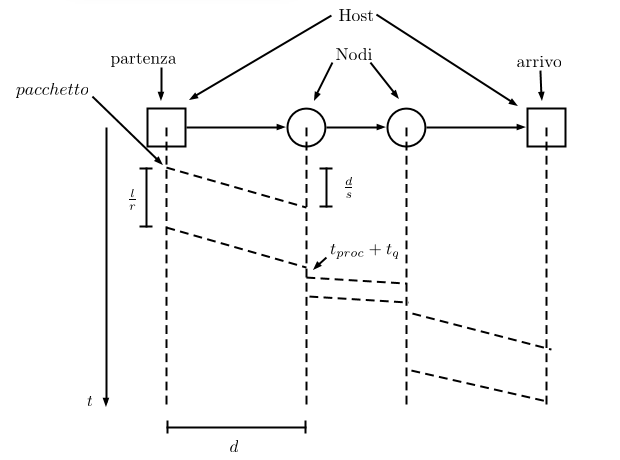
\includegraphics[scale=0.5]{img/reti.png}
\end{center}
\end{document}